% !TEX root = thesis.tex

\chapter{TraffickCam}
\label{ch:3}
Sex trafficking has become more prevalent as the Internet provides new avenues for the recruiting, advertisement and sales of sexual services [7]. We explore the opportunities of a highly connected world to build tools to fight sex trafficking. We particularly focus on understanding places where large scale image collection and analysis offers new investigative tools.

Images are a common way to advertise sex services. Images are interesting from an investigative standpoint because they connect the person in the image to the location where the image was taken. Therefore, they can help to characterize where a particular person was at different times. In the context of a sex trafficking investigation, this can be used to
directly confirm that a person was in different states or countries. Among other things, this can change the set of laws under which a trafficker can be prosecuted.

We aim to create a database of hotel room images that an investigator can use to understand the pictures they may acquire during a sex trafficking investigation. We build a dataset from publicly shared imagery on hotel booking sites, as well as from a smartphone app to crowd-sourcing the collection of pictures of hotel rooms. The crowd-sourcing option
takes advantage of large scale trends in how people use social media; approximately 350 million photos are uploaded daily to Facebook. Tapping into this already common behavior creates the potential to rapidly create a relatively comprehensive, distributed,
and continually updated resource that details the current appearance of hotel rooms worldwide.

\section{Dataset Creation}
In order to have the highest likelihood of finding a good feature match between a investigator's query image and the images in our dataset, our dataset should have as many images of as many rooms in as many hotels as possible. Additionally, it should have images from as many different times as possible. Hotels regularly renovate and change their internal appearance, meaning that photographs in our dataset may become outdated. These outdated images may still be valuable, however, in pinpointing the time frame in which an individual was trafficked (e.g., ``This photograph was taken before the 2015 renovations, which means the person in the photograph was a minor at the time the advertisement was placed.'').

\section{Crowd-sourced Image Collection}
\begin{figure*}[ht!]
  \begin{center}
    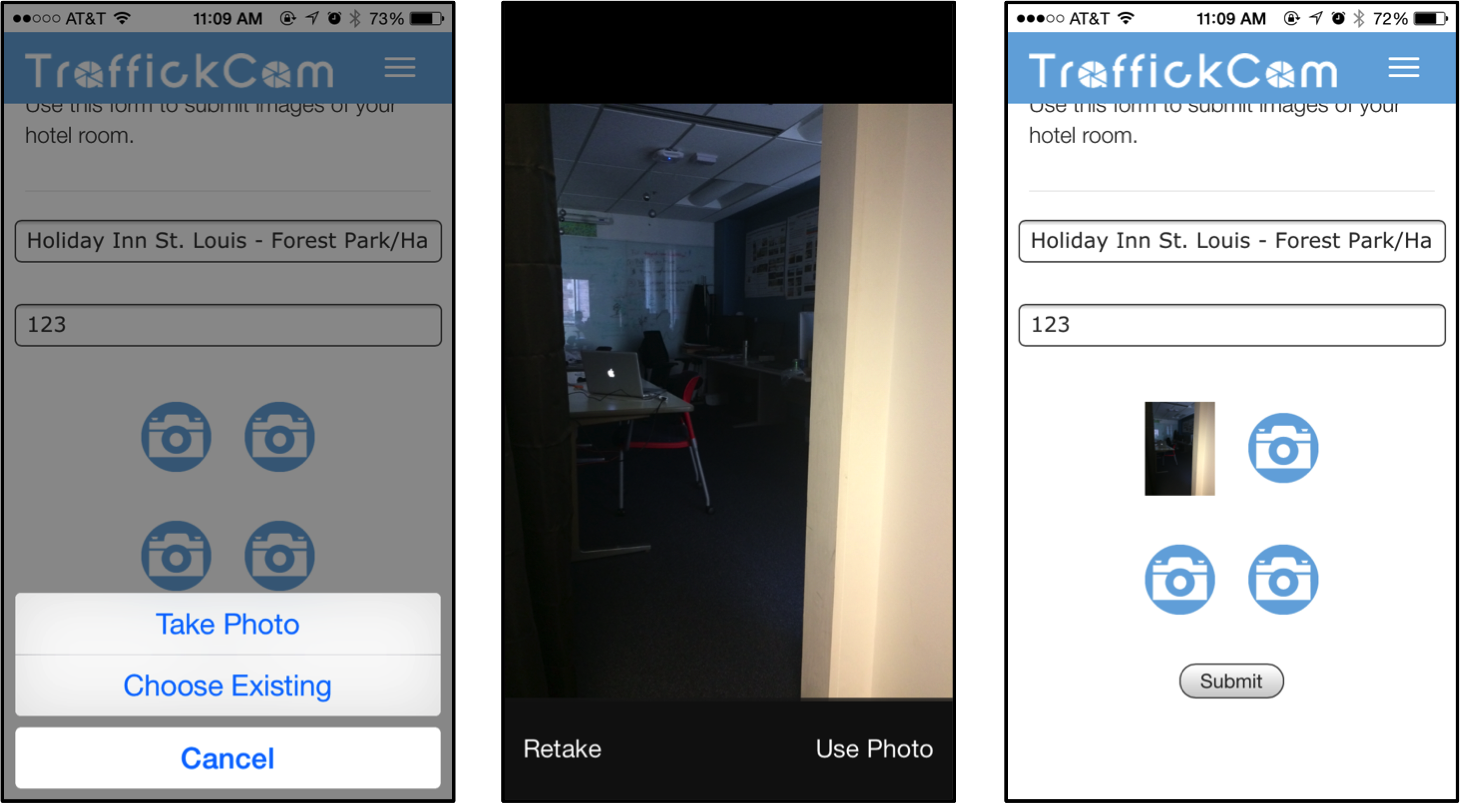
\includegraphics[width=\textwidth]{figures/chapter3/appScreenshots.png}
  \end{center}
  \caption[Smartphone app screenshots.]{Screenshots of the smartphone app, TraffickCam, that allows anyone to contribute to the database. The app is designed to require minimal user time and to protect the user's identity.}
  \label{fig:appScreenshots}
\end{figure*}

We take two approaches to populating our dataset of hotel room images. First, we utilize already existing datasets of hotel room images used for marketing and travel sales. In particular, we keep track of the millions of images made available through
Expedia’s Affiliate Network API (http://developer.ean.com/) and create a reference in our database to the original data and its associated metadata. These photos, however, are often provided by the hotels themselves and may not present a comprehensive view of the hotel itself (e.g., only the nicest rooms from good angles in the best lighting). They may also
not be updated following renovations. Both of those flaws would be problematic if these photographs were the only representations our dataset had of these hotels. 

To supplement the images captured from existing datasets, we have created a smartphone crowd-sourcing application named TraffickCam, which allows travellers to upload their own photographs of a hotel room. This application is shown in Figure~\ref{fig:appScreenshots}. Users are asked to provide minimal information regarding the photo -- the name of the hotel they're staying in and their room number, along with images of the room.

The application, called TraffickCam, is available from the iOS and Android stores, in addition to being accessible via any modern browser at \url{http://traffickcam.org}.

Examples of images from both the Expedia dataset and the TraffickCam dataset, as well as representative images that law enforcement might upload to the TraffickCam system can be seen in Figure~\ref{fig:example_ims}.

\begin{figure*}[ht!]
  \begin{center}
  \begin{subfigure}[b]{\textwidth}
    \centering
    ~~~~~~~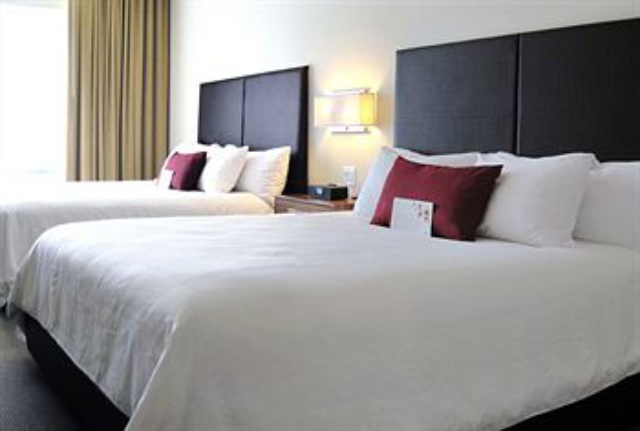
\includegraphics[width=.25\columnwidth]{figures/chapter3/expediaIms/1.jpg}
    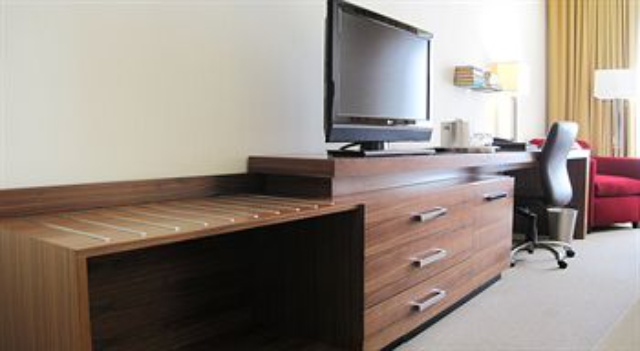
\includegraphics[width=.25\columnwidth]{figures/chapter3/expediaIms/2.jpg}
    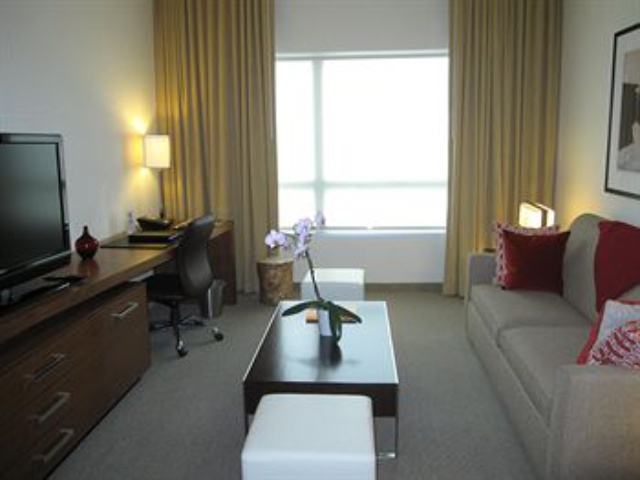
\includegraphics[width=.25\columnwidth]{figures/chapter3/expediaIms/3.jpg}
    \newline
    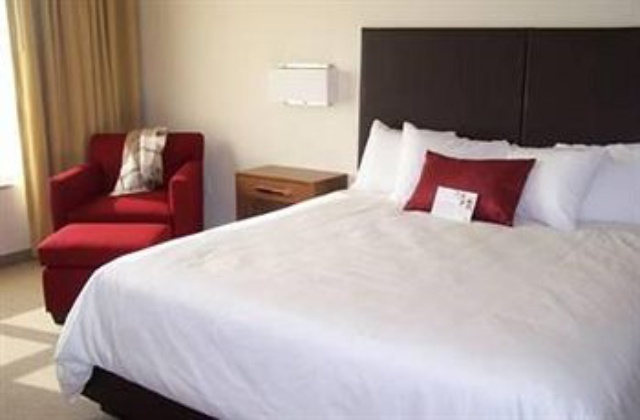
\includegraphics[width=.25\columnwidth]{figures/chapter3/expediaIms/4.jpg}
    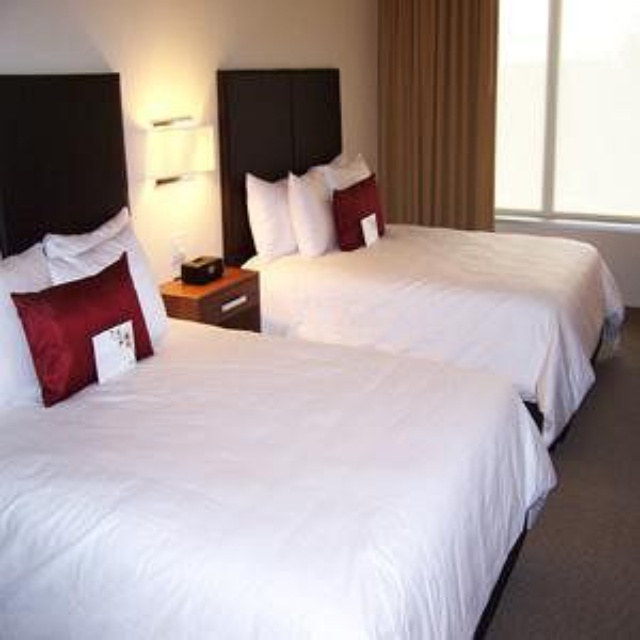
\includegraphics[width=.25\columnwidth]{figures/chapter3/expediaIms/5.jpg}  
    
\includegraphics[width=.25\columnwidth]{figures/chapter3/expediaIms/6.jpg} 
    \caption{Expedia Images}
  \end{subfigure}
  
  \begin{subfigure}[b]{\textwidth}
    \centering
    ~~~~~~~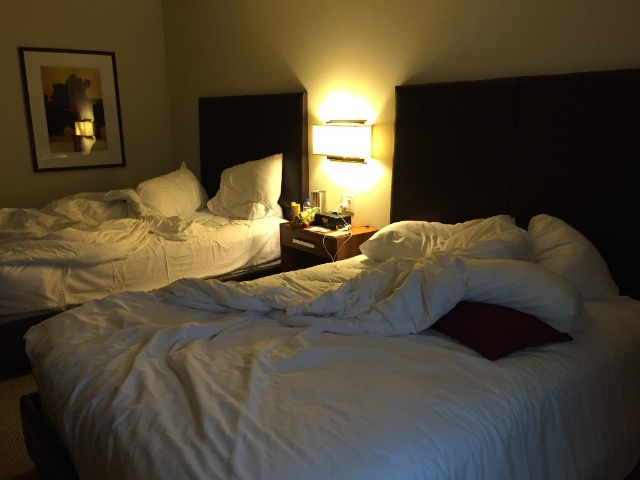
\includegraphics[width=.25\columnwidth]{figures/chapter3/traffickCamIms/1.jpg}
    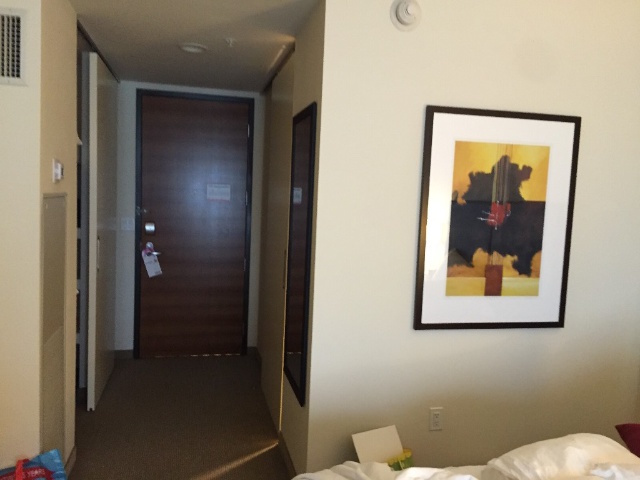
\includegraphics[width=.25\columnwidth]{figures/chapter3/traffickCamIms/2.jpg}
    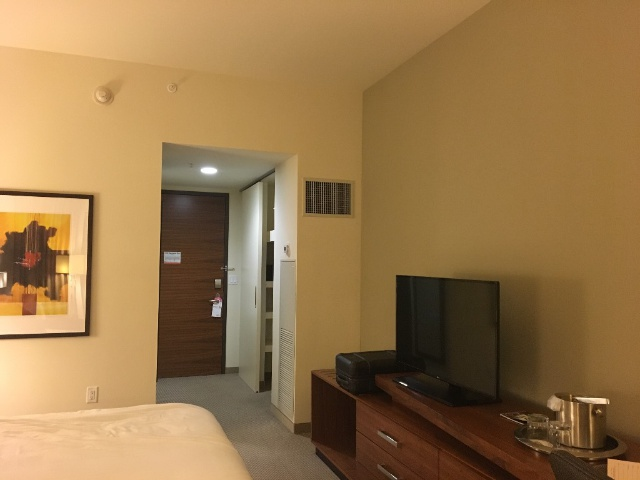
\includegraphics[width=.25\columnwidth]{figures/chapter3/traffickCamIms/3.jpg}
    \newline
    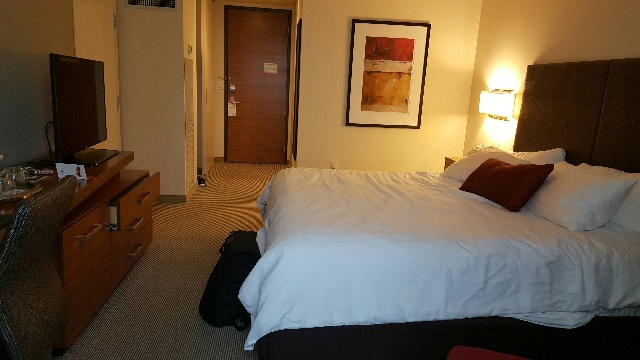
\includegraphics[width=.25\columnwidth]{figures/chapter3/traffickCamIms/4.jpg}
    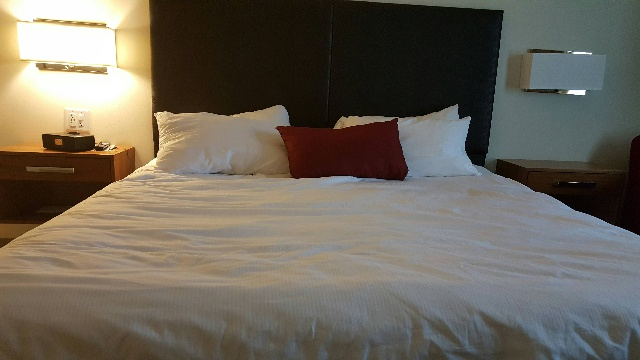
\includegraphics[width=.25\columnwidth]{figures/chapter3/traffickCamIms/5.jpg}  
    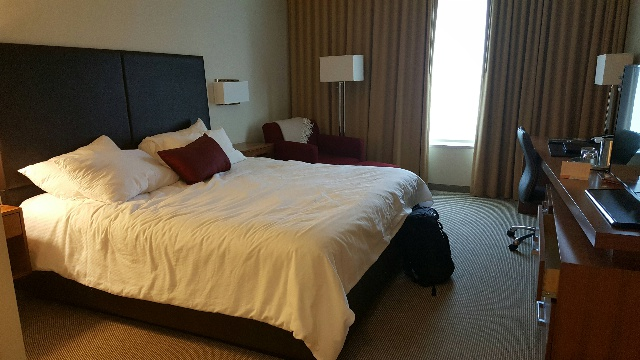
\includegraphics[width=.25\columnwidth]{figures/chapter3/traffickCamIms/6.jpg}  
    \caption{TraffickCam Images}
  \end{subfigure}
  
  \begin{subfigure}[b]{\textwidth}
  \centering
    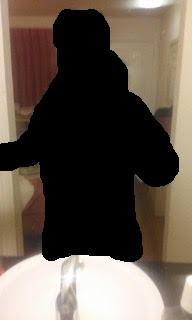
\includegraphics[height=120px]{figures/chapter3/backpage/3.jpg}
    ~~~~~~
    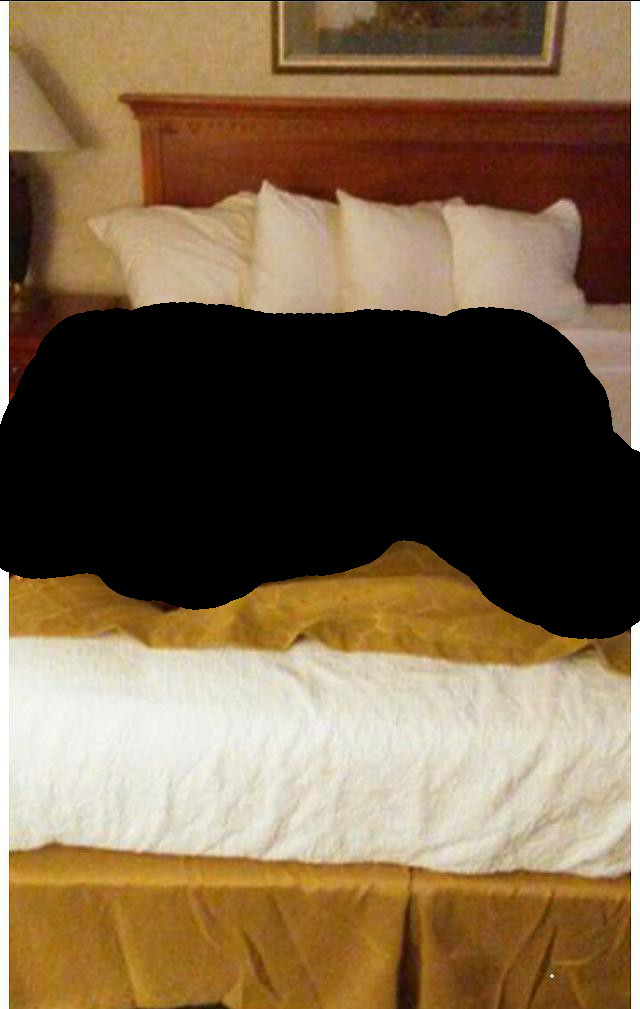
\includegraphics[height=120px]{figures/chapter3/backpage/1.jpg}
    ~~~~~~
    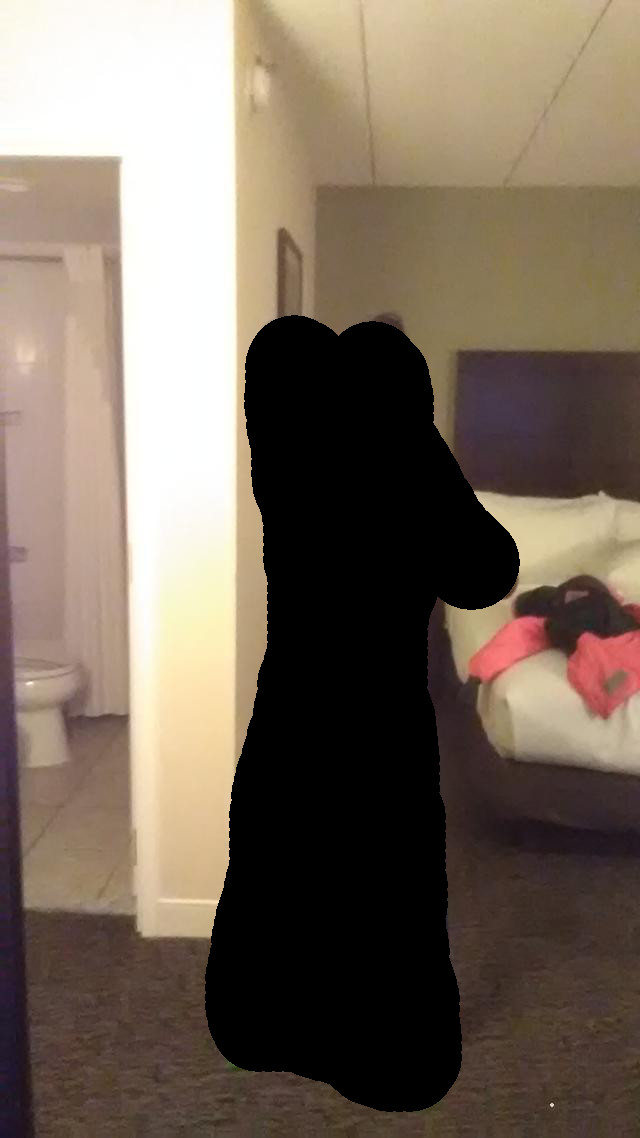
\includegraphics[height=120px]{figures/chapter3/backpage/2.jpg}
    \caption{Example Censored Query Images from Law Enforcement}
  \end{subfigure}
  
  \caption[Example images from TraffickCam and Expedia.]{The top set of images are from Expedia and the middle set of images taken by TraffickCam users at the same hotel. The bottom set of images are censored versions of the types of images that might be provided by law enforcement. These examples demonstrate the discrepancy in the types of photos provided by Expedia, by the TraffickCam app and by law enforcement.}
  \label{fig:example_ims}
  \end{center}
\end{figure*}

\section{Dataset Scope}
The present TraffickCam database includes 1,629,505 images from 150,289 unique hotels. Of these hotels, 131,244 hotels have only Expedia images, 15,242 have only TraffickCam images, and 10,742 hotels have both TraffickCam and Expedia images.

While the TraffickCam application purposefully collects no identifiable information about users to protect them from any legal action, we are able to estimate the number of users per hotel by the timestamp of the images uploaded -- the application asks users for a set of four images, so we assume images that are disjoint in time are from different users.

\section{Implementation Details}
We have implemented a RESTful API in Python Django, a web framework for rapid web development. Django handles the interaction between the server side code, web front end code, MySQL database and Apache web server. Test, stage and production Ubuntu environments are hosted through Amazon Web Services.

The iOS app, available through the Apple App Store, is simply a container that renders an HTML5+jQuery+AJAX web application hosted on~\url{https://traffickcam.org}, rather than a full native application. This allows for rapid development and easy exploration of different user experience choices (e.g., different motivational messages to display to users upon submission). The Android application is a native application available on the Google Play store.

\section{Application Statistics}
Since TraffickCam was released in December of 2015, there have been 68,700 installations on iOS devices and 28,500 installations on Android devices. These installations are primarily from users in the United States, where the search tool will first be deployed for law enforcement, but also include several thousand installations each from Europe and Asia. On average since the advertised release of the TraffickCam applications for iOS and Android in June of 2016, users have submitted just over 530 images a day.